\documentclass{homework}
\usepackage{marvosym}
\usepackage{hyperref}
\usepackage{color}
\usepackage{caption}
\usepackage{float}

\course{Algorithmische Bioinformatik}
\semester{Wintersemester 2012 / 2013}
\no{10}
\date{Montag, dem 7. Januar 2013}
\author{Stefan Meißner (4279113) und Niels Hoppe (4356370)}
\tutorial{Dienstag 08:00 - 10:00}
\tutor{Alena van Bömmel (Übungsgruppe 3)}

\begin{document}
\maketitle
\begin{enumerate} 

\aufgabe{Lander-Waterman-Statistik}{\qquad}

\begin{enumerate}
\item 
\item 
\end{enumerate}

\aufgabe{Praktisches Assembly}{100}

\begin{enumerate}
\item 
Wenn die Sequenzen per Zufall generiert wurden, kann es sich um jeden beliebigen Organismus handeln.
\item 
Nach der Vorverarbeitung durch \textit{velveth}, erzeugt \textit{velvetg} folgende Ausgabe:
\begin{verbatim}
Final graph has 886 nodes and n50 of 624, max 2162, 
 total 122076, using 0/10000 reads
\end{verbatim}
Nicht ganz klar ist, was jetzt als Node bezeichnet wird? In der contigs.fa gibt es genau $886 / 2 = 443$ Sequenzen.
\item 
Wie im Manual beschrieben, erstellen wir das gewichtete Histogramm mit R:
\begin{verbatim}
library(plotrix)
data = read.table("stats.txt", header=TRUE)
hist(data$short1_cov, breaks=1000)
weighted.hist(data$short1_cov, data$lgth, breaks=0:50)
\end{verbatim}
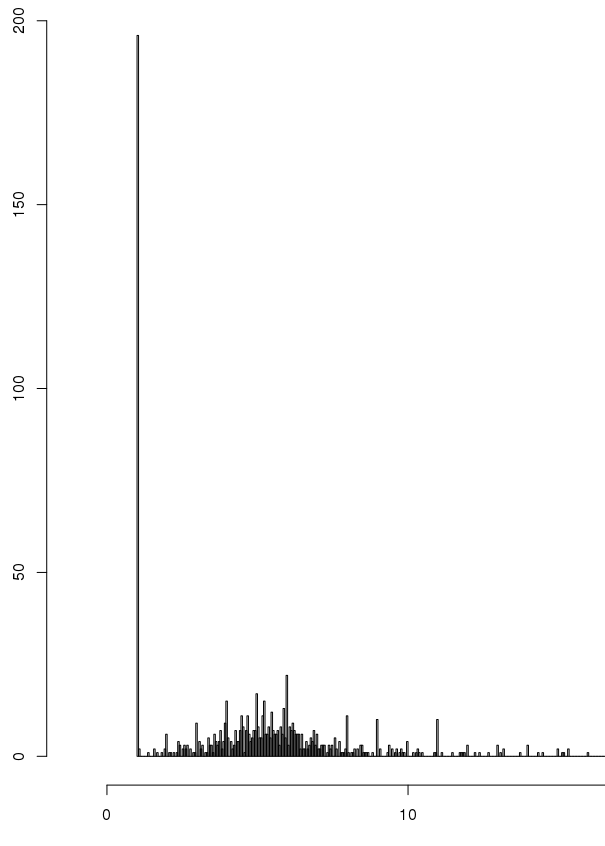
\includegraphics[scale=0.3]{../data/aufg_36_3_a}
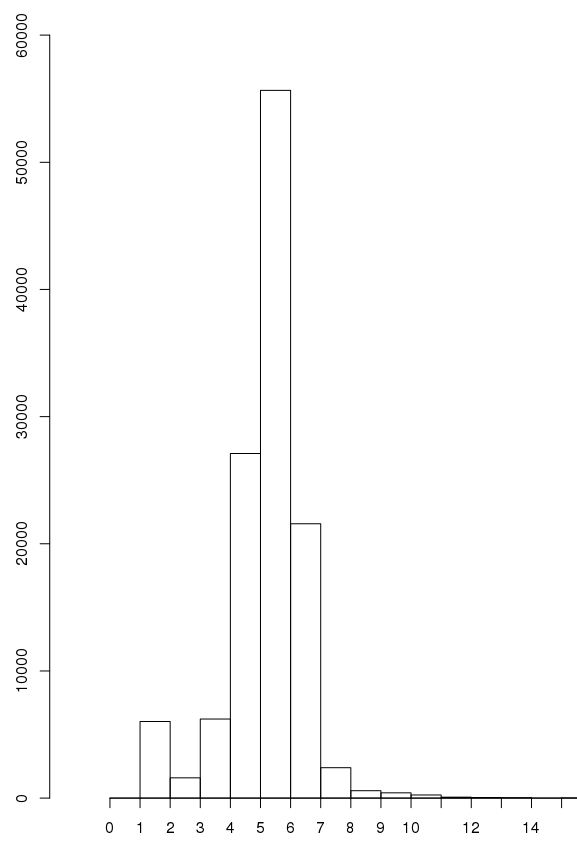
\includegraphics[scale=0.3]{../data/aufg_36_3_b}

Wir setzen den Cov\_{}Cutoff bei 4.
\item 
Diesmal gibt es folgende Ausgabe:
\begin{verbatim}
Final graph has 228 nodes and n50 of 1144, max 2925,
 total 107933, using 0/10000 reads
\end{verbatim} 
\item 
N50 Definition nach Jeremy Leipzig:\\
\textit{N50 length is the length of the shortest contig such that the sum of contigs of equal length or longer is at least 50\% of the total length of all contigs.}\\
D.h. je Höher dieser Wert ist, desto höher ist die Qualität des Assamblies. Die Contigs mit dem Cov\_{}Cutoff 4 sind also fast doppelt so lang, da hier Lesefehler bereinigt sind. Einen noch größeren N50 Wert lässt sich durch den Parameter  \textit{cov\_{}cutoff auto} erzielen:
\begin{verbatim}
[0.101757] Estimated Coverage cutoff = 2.644231
Final graph has 271 nodes and n50 of 1147, max 3921,
 total 114404, using 0/10000 reads
\end{verbatim}
\item 
\begin{verbatim}
Simple repeats: 272 10275 bp 1.03 %
\end{verbatim}

\item 
Hier erhält man eine sehr lange Liste (127 predicted genes), die wie folgt begint:
\begin{verbatim}
Gn.Ex Type S .Begin ...End .Len Fr Ph I/Ac Do/T CodRg P.... Tscr..
----- ---- - ------ ------ ---- -- -- ---- ---- ----- ----- ------

 1.02 Term -    174    110   65  1  2   47   35   127  -nan   4.01
 1.01 Init -   8030   8021   10  2  1  127    3     0  -nan  -1.66
 1.00 Prom -  13209  13170   40                               2.02
\end{verbatim}
\item 
Keine Ahnung, komische Aufgabenstellung...Es gibt ja durch die Simulation keine Referenzsequenz. 
\item 
\end{enumerate}

\aufgabe{Lowess Normalisierung}{70}

\begin{verbatim}
# einlesen der Daten, Teilaufgabe (i)
data <- read.delim("wood_data.txt")

# Einige Plot Eigenschaften, damit die Anzeige schoen ist
# - Fenster initialisieren
# - Plotten in einer 5x4 Matrix
dev.new()
op <- par(no.readonly = TRUE)
dev.off()
op
par(mfrow=c(5,4))


# beginne bei Spalte 3 und betrachte jeweils 2 Spalten
# Teilaufgabe (ii)
for (i in seq(3,(length(data)-1),2)){
		m <- log(x=as.vector(as.matrix(data[i]/data[i+1])), base=2)
		a <- 0.5*log(x=as.vector(as.matrix(data[i]*data[i+1])), base=2)
	
		# entferne alle unbrauchbaren Werte (NA, NaN, Inf, -Inf)
		# m <- m[!is.nan(m)]
		# m <- m[!is.na(m)]
		m <- m[is.finite(m)]
		a <- a[is.finite(a)]
		
		column = names(data)[i]				
		plot(y=m, x=a, type = "p", main=column)	

        # Teilaufgabe (iii)
		lines(x=seq(1,15), y=seq(1,15)*0 + mean(m), col="blue")
		# Fensterbreite fuer lowess = 2/3 (default)
		# zu kleine Werte fuehren zu vielen kleinen Ausschlaegen
		# bei zu grossen Werten wird zu viel geglaettet
		lines(lowess(y=m, x=a, f=0.66), col="red")
}
\end{verbatim}

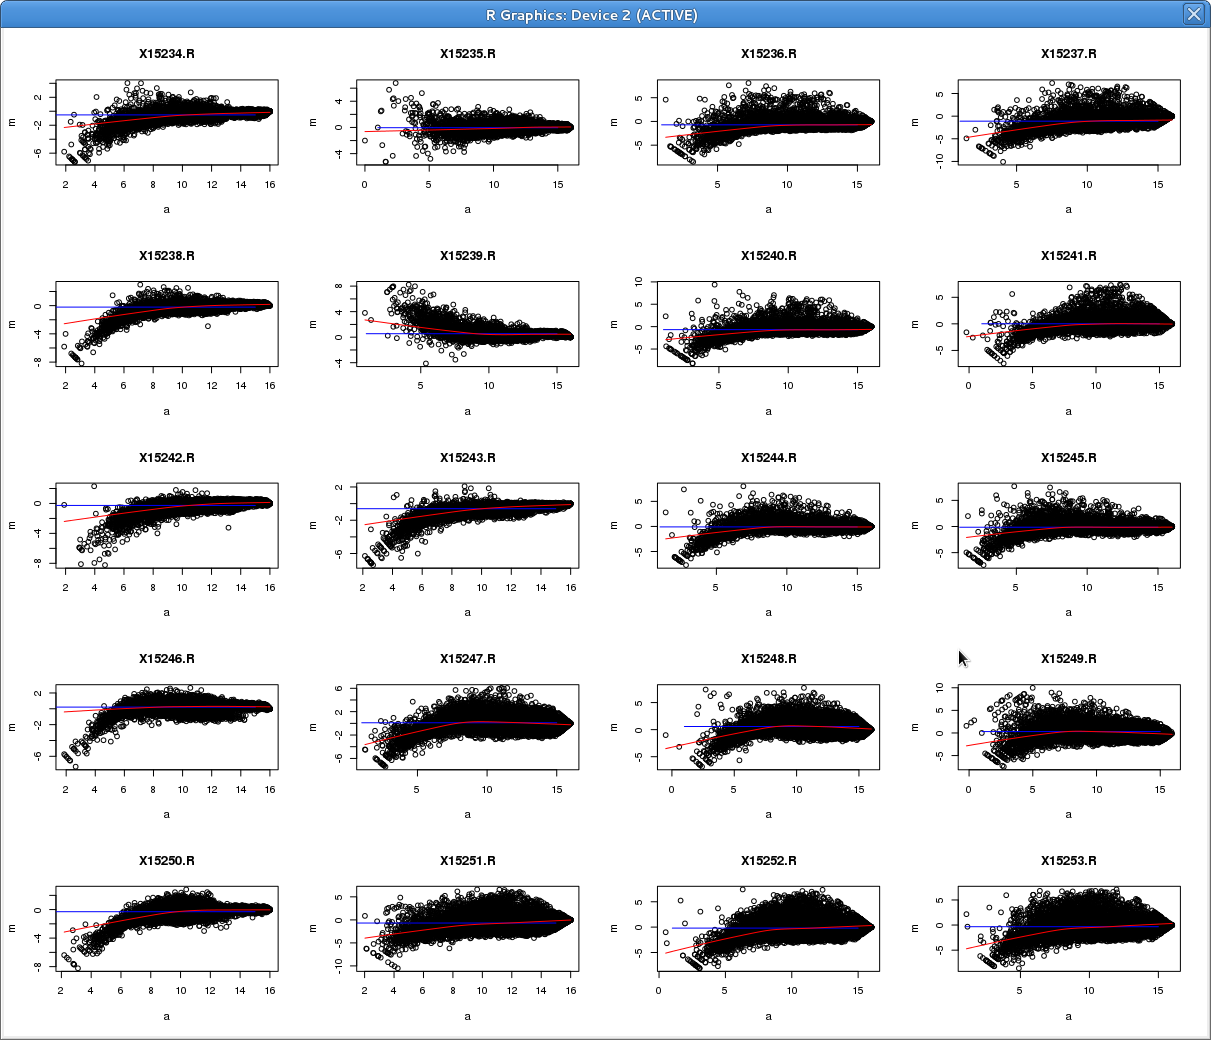
\includegraphics[scale=0.3]{../data/aufg_37}

\aufgabe{Quantilnormalisierung}{50}

\begin{enumerate}
\item 
\item 
\item
\item
\end{enumerate}

\end{enumerate}
\end{document}
